% vim:autoindent:set textwidth=78:

\section{Trabajando con proyecciones}\label{label_projections}
\index{Projections!working with}

% when the revision of a section has been finalized, 
% comment out the following line:
%\updatedisclaimer

QGIS permite a los usuarios definir un SRC (Sistema de Referencia de
Coordenadas) global y un SRC con \'ambito de proyecto para capas sin un SRC predefinido. Tambien permite al
usuario definir sistemas de referencia de coordenadas personalizados y soporta proyecciones de capas
vectoriales al vuelo(OTF, on the fly). Todas estas caracter\'{\i}sticas permiten al usuario mostrar
capas con diferentes SRC y sobreponerlos apropiadamente.

\subsection{Descripci\'on general del soporte de proyecciones}\label{label_projoverview}

QGIS tiene soporte para aproximadamente 2,700 SRC conocidos. Las definiciones para 
cada uno de estos SRC est\'a almacenada en una base de datos SQLite database que es instalada con
QGIS. Normalmente no tiene  necesidad de manipular la base de datos directamente. De hecho,
hacerlo puede causar que el soporte de proyecciones falle. Los SRC personalizados son almacenados en una
base de datos de usuario. Vea la secci\'on \ref{sec:customprojections} para 
informaci\'on en el manejo de sus sistemas de referencia de coordenadas personalizados.

Los SRC disponibles en QGIS est\'an basados en los definidos por la
EPSG\index{EPSG} y son abstraidos en gran medida de la tabla spatial\_references 
en PostGIS\index{PostGIS} version 1.x. Los identificadore EPSG est\'an
presentes en la base de datos y pueden ser usados para especificar un SRC en QGIS.

Con el fin de usar proyecci\'on al vuelo(OTF), sus datos deden contener informaci\'on acerca de su
sistema de referencia de coordenadas o debe definir un SRC global, de capa o
de proyecto. Para capas de PostGIS QGIS usa el identificador de referencia espacial
que fue especificado cuando la capa fue creada. Para datos soportados
por OGR, QGIS depende de la presencia de una manera de formato de especificar
el SRC. En el caso de shapefiles, esta manera es un archivo conteniendo la especificacion Well
Known Text (WKT)\index{WKT} de el CRS. El archivo de proyecci\'on
tiene el mismo nombre base que el shapefile y una extensi\'on prj. Por ejemplo, un
shapefile llamado \filename{alaska.shp} tendr\'{\i}a un nombre de archivo de proyecci\'on
correspondiente \filename{alaska.prj}.

\subsection{Especificando una proyecci\'on}
\index{Projections!specifying}
\label{sec:projection-specifying}

QGIS ya no establece el SRC del mapa al sistema de referencia de coordenadas de la
primera capa cargada. Cuando comienza una sesi\'on de QGIS con capas que no tienen
un CRS, necesita controlar y definir la dedinici\'on de SRC para estas
capas. Esto puede ser realizado globalmente o en el proyecto en la pesta\~na \tab{SRC} bajo
\mainmenuopt{Editar} > \dropmenuopttwo{mActionOptions}{Opciones} (Gnome, OSX) 
or \mainmenuopt{Configuraci\'on} > \dropmenuopttwo{mActionOptions}{Opciones} (KDE, Windows). 
See Figure~\ref{fig:crsdialog}. 

\begin{itemize}
\item \checkbox{Preguntar SRC} 
\item \checkbox{Usar el SRC predeterminado del proyecto}
\item \checkbox{Usar el SRC global predeterminado mostrado abajo}
\end{itemize}

El SRC global predeterminado \texttt{proj=longlat +ellps=WGS84 +datum=WGS84
+no\_defs} viene predefinido en QGIS pero puede ser cambiado, y la nueva definici\'on
ser\'a almacenada para sesiones subsecuentes de QGIS.    

\begin{figure}[ht]
   \begin{center}
   \caption{Pesta\~na SRC en el di\'alogo de opciones de QGIS \nixcaption}\label{fig:crsdialog}\smallskip
   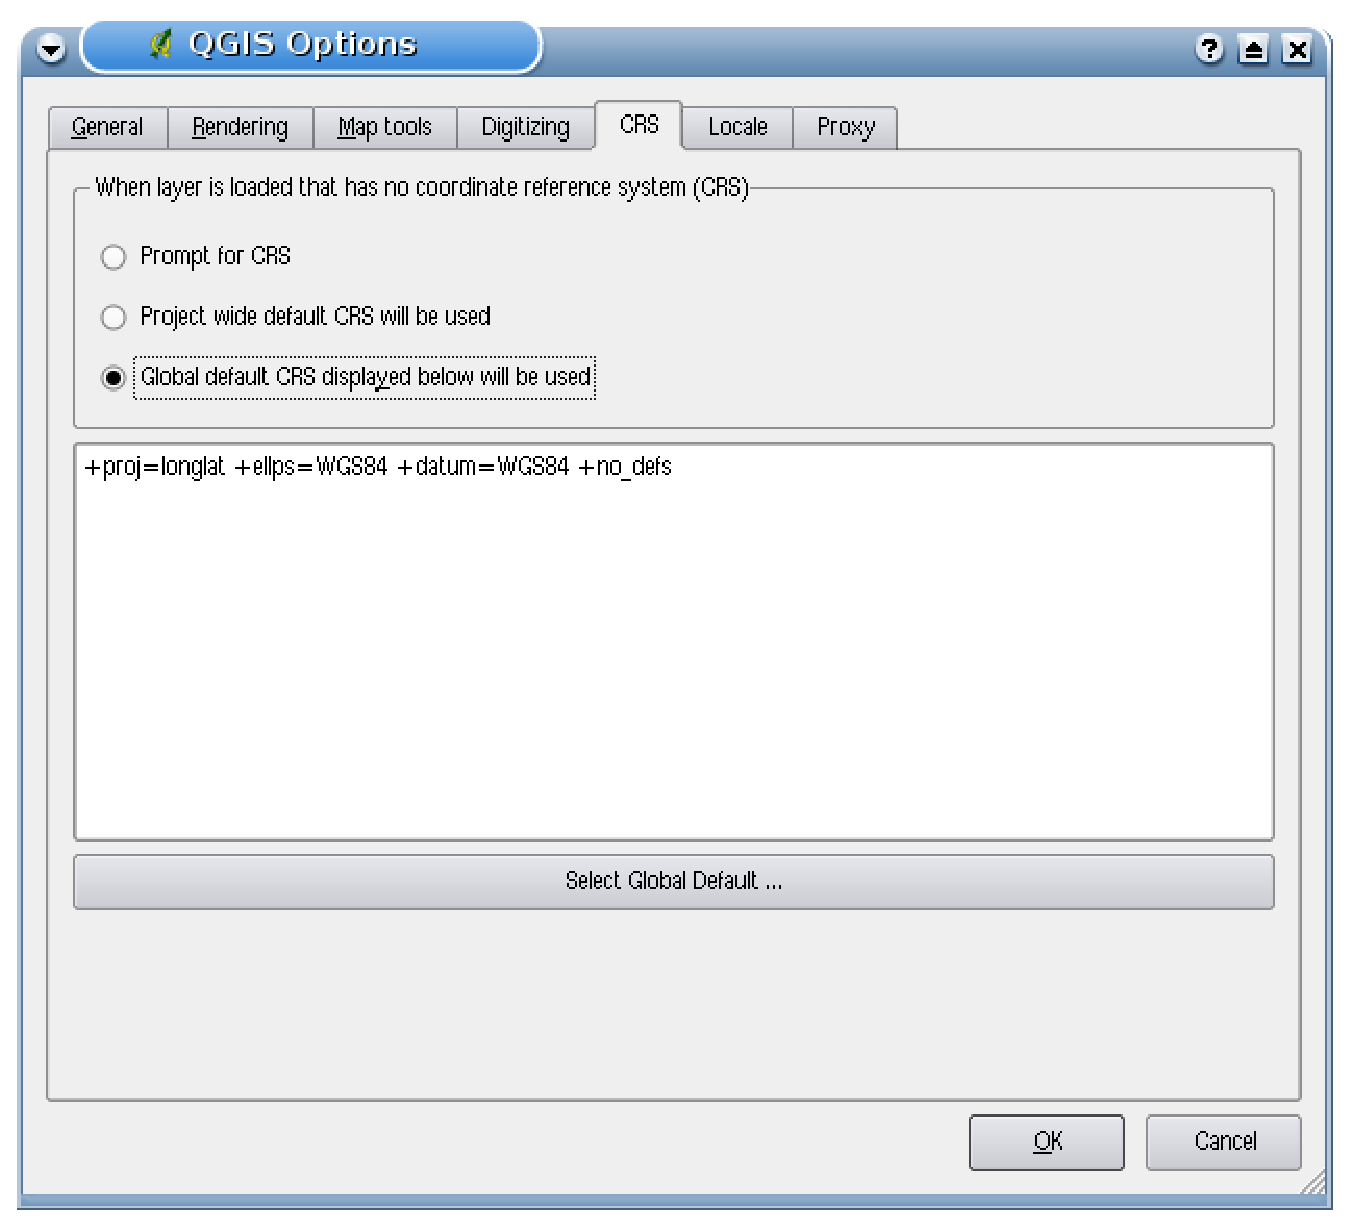
\includegraphics[clip=true, width=12cm]{crsdialog}
\end{center}
\end{figure}

Si quiere definir el sistema de referencia de coordenadas para una capa espec\'{\i}fica
sin informaci\'on de SRC, puede hacerlo en la pesta\~na \tab{General} del
di\'alogo de propiedades raster (\ref{label_generaltab}) y vector (\ref{vectorgeneraltab}).  
Si su capa ya tiene un SRC definido, ser\'a
mostrada como en la figure~\ref{fig:vector_symbology}.

\subsection{Definir proyecci\'on al vuelo(OTF)}\label{label_projstart}

QGIS no tiene activo la proyecci\'on al vuelo en forma predeterminada, y esta funci\'on actualmentes solo
es soportada para capas vectoriales. Para usar proyecci\'on al vuelo, debe
abrir el di\'alogo \dropmenuopttwo{mActionOptions}{Propiedades del proyecto}, seleccionar un
SRC y activar la caja de verificaci\'o \checkbox{Activar transformaci\'on de SRC al vuelo}.
Hay dos forma de abrir el di\'alogo:

\begin{enumerate}
\item Seleccionando \dropmenuopttwo{mActionOptions}{Propiedades del proyecto} del men\'u
\mainmenuopt{Editar} (Gnome, OSX) or \mainmenuopt{Configuraci\'on} (KDE, Windows).
\item Clic en el \'{\i}cono \toolbtntwo{mIconProjectionDisabled}{proyector} de la
esquina inferior derecha de la barra de estado.
\end{enumerate}

Si tiene una capa cargada, y quiere activar proyecci\'on al vuelo, la
mejor pr\'actica es abrir la pesta\~na \tab{Sistema de referencia de coordenadas} del
di\'alogo \dialog{Propiedades del proyecto}, seleccionar el SRC de la capa actualmente cargada,
y activar la caja de verificaci\'on \checkbox{Activar transformaci\'on de SRC al vuelo}. El
\'{\i}cono \toolbtntwo{mIconProjectionEnabled}{proyector} mostrar\'a un gancho verde
y todas las capas vectoriales subsecuentemente cargadas ser\'an proyectadas al vuelo a el
SRC definido.
 
La pesta\~na \tab{Sistema de referencia de coordenadas} del di\'alogo \dialog{Propiedades del proyecto}
contiene 4 importantes componentes como se muestra en la figura
\ref{fig:projections} y descrita abajo.

\begin{figure}[ht]
   \begin{center}
   \caption{Di\'alogo proyecci\'on \nixcaption}\label{fig:projections}\smallskip
   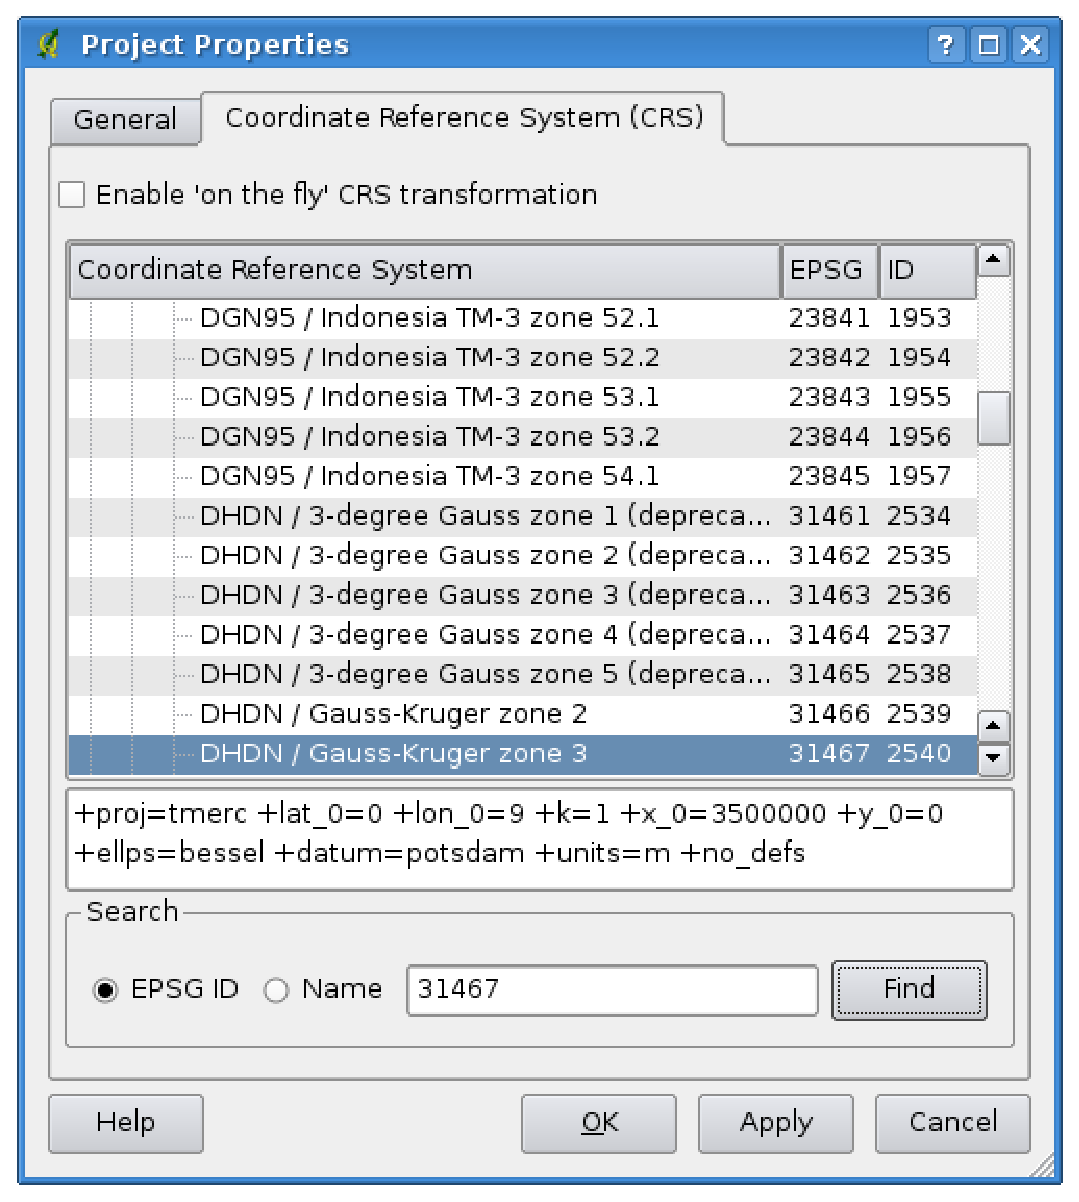
\includegraphics[clip=true, width=12cm]{projectionDialog}
\end{center}  
\end{figure}

\begin{enumerate}
\item \textbf{Activar transformaci\'on de SRC al vuelo}\index{Projections!enabling} -
esta caja de verificaci\'on es usada para activar o desactivar la proyecci\'on al vuelo. Cuando est\'a desactivado, cada
capa es dibujada usando las coordenadas como son leidad del conjunto de datos. Cuando est\'a activo,
las coordenadas de cada capa son proyectados al sistema de referencia de coordenadas
definido para el mapa.
\item \textbf{Sistema de referencia de coordenadas} - esta es una lista de todas las SRC
soportados por QGIS, incluyendo Geogr\'aficas, Projectadas and sistemas de referencia
de coordenadas personalizados. Para usar un SRC, seleccionelo de la lista expandiendo
el nodo apropiado y seleccionando el SRC. El SRC activo es preseleccionado.
\item \textbf{Texto Proj4} - este es la cadeba SRC usada por el motor de proyecciones Proj4.
Este texto es de solo lectura y se provee para prop\'ositos de
informaci\'on.
\item \textbf{Buscar} - si usted conoce el identificador EPSG o el nombre 
para un sistema de referencia de coordenadas, puede usar la funcionalidad buscar para encontrarla.
Escriba el identificador y haga clic en \button{Encontrar}.
\item \textbf{SRC usados recientemente} - si tiene SRC espec\'{\i}fico que usa frecuentemente 
en su trabajo diario de GIS, este ser\'a mostrado como botones de 'acceso r\'apido' 
en la parte de abajo del di\'alogo de proyecci\'on. Haga clic en uno de estos botones para seleccionar
el SRC asociado.
\end{enumerate}

\begin{Tip}
\caption{\textsc{Di\'alogo de propiedades del proyecto}}
\qgistip{
Si abre el di\'alogo de \dialog{Propiedades del proyecto} desde el
men\'u \mainmenuopt{Editar} (Gnome, OSX) or \mainmenuopt{Configuraci\'on} 
(KDE, Windows), debe hacer clic en la pesta\~na \tab{Sistema de referencia de coordenadas
} para ver las configuraciones SRC. Abriendo el di\'alogo desde el
\'{\i}cono \toolbtntwo{mIconProjectionEnabled}{proyector} traer\'a
la pesta\~na \tab{Sistema de referencia de coordenadas} al frente.
}
\end{Tip}

\subsection{Sistema de referencia de coordenadas personalizado}\label{sec:customprojections}
\index{Projections!custom}

Si QGIS no provee el sistema de referencia de coordenadas que necesita, puede
definir SRC personalizado. Para definir un SRC, selecciones
\dropmenuopttwo{mIconNew}{SRC personalizado} desde el men\'u \mainmenuopt{Editar} 
(Gnome, OSX) or \mainmenuopt{Configuraci\'on} (KDE, Windows).
Los SRC personalizados son almacenados en su base de datos de usuario. Adicionalmente a su
SRC personalizado, esta base de datos tambien contiene sus marcadores espaciales y otros datos personalizados. 

\begin{figure}[ht]
   \begin{center}
   \caption{Di\'alogo de SRC personalizado \nixcaption}\label{fig:customprojections}\smallskip
   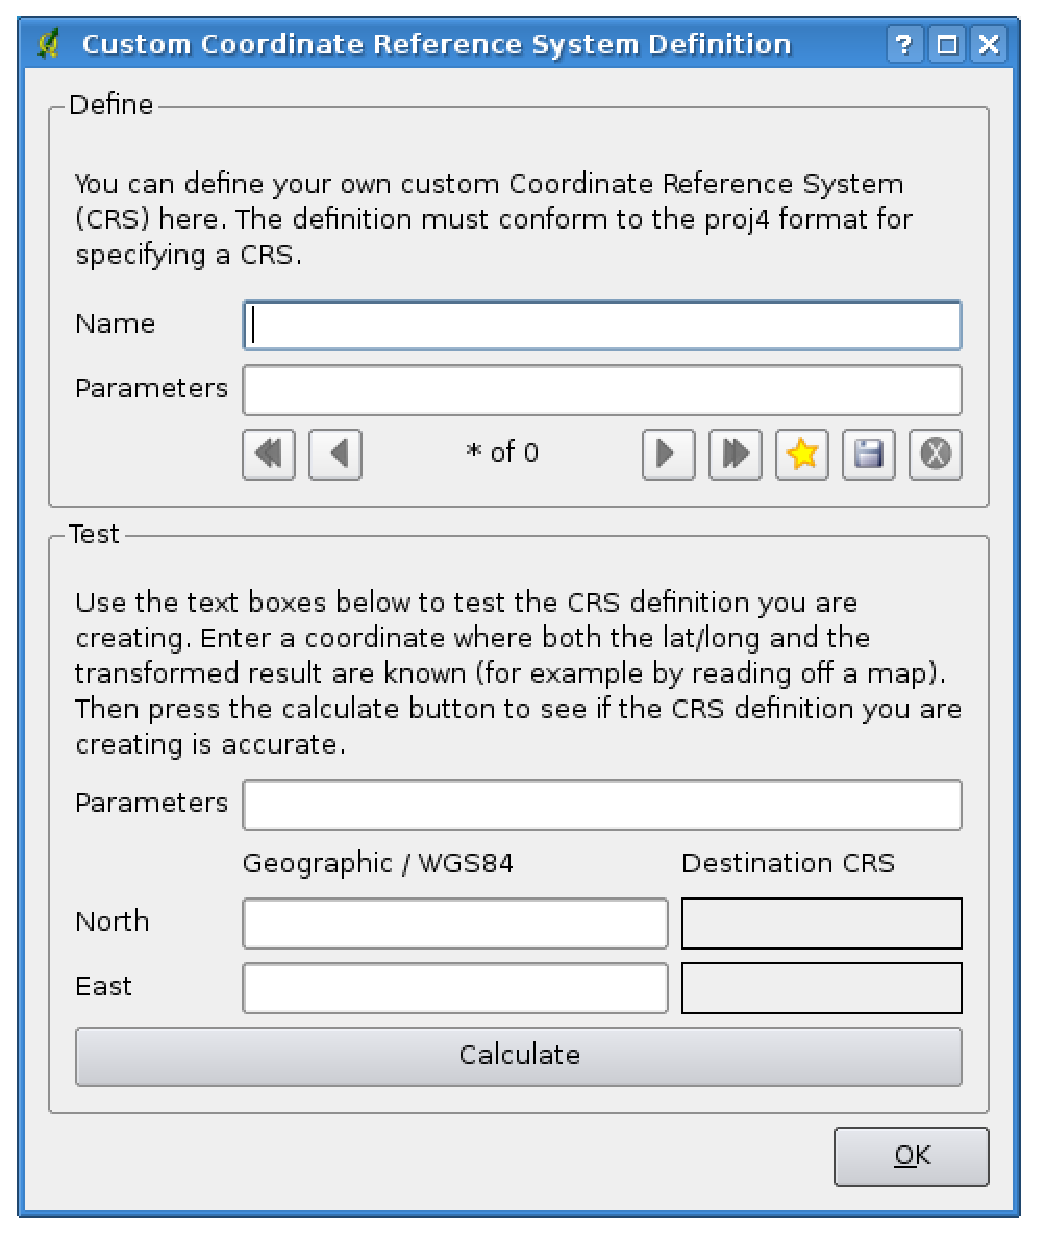
\includegraphics[clip=true, width=12cm]{customProjectionDialog}
\end{center}  
\end{figure}

Definir un CRS personalizado en QGIS requiere una buena comprensi\'on de la
librer\'{\i}a de proyecciones Proj.4. Para comenzar, rem\'{\i}taze a Cartographic Projection Procedures
for the UNIX Environment - A User's Manual by Gerald I. Evenden, U.S.
Geological Survey Open-File Report 90-284, 1990 (available at \url{ftp://ftp.remotesensing.org/proj/OF90-284.pdf}).
Este manual describe el uso del \usertext{proj.4} y las utilerias de
l\'{\i}nea de comandos. Los par\'ametros cartogr\'aficos usados con \usertext{proj.4} son
descritos en el manual de usuario, y son los mismos que los usados por QGIS. 

El di\'alogo \dialog{Definici\'on de sistemas de referencia de coordenadas personalizados} requiere
solo dos par\'ametros para definir un SRC de usuario: 
\begin{enumerate}
\item un nombre descriptivo y
\item los par\'ametros cartogr\'aficos en formato PROJ.4.
\end{enumerate}
Para crear un nuevo SRC, haga clic en el bot\'on \toolbtntwo{mIconNew}{Nuevo} y escriba un
nombre descriptivo y los par\'ametros SRC. Despues de eso puede guardar su SRC haciendo clic
en el bot\'on \toolbtntwo{mActionFileSave}{Guardar}.

Note que los \guilabel{Par\'ametros} deben comenzar con un bloque \usertext{+proj=},
para representar el nuevo sistema de referencia de coordenadas.

Puede probar los par\'ametros de se SRC para ver si dan resultados sanos
haciendo clic en el bot\'on \button{Calcular} dentro del bloque \guiheading{Probar} 
y pegando sus par\'ametros SRC dentro del
campo \guilabel{Par\'ametros}. Entonces capture los valores conocidos WGS 84 latitud y longitud
en los campos \guilabel{Norte} y \guilabel{Este} respectivamente. 
Haga clic en \button{Calcular} y compare los resultados con los valores conocidos en
sus sistema de referencia de coordenadas. 

